\chapter{Kiến trúc của framework Ruby on Rails}
Giới thiệu kiến trúc tổng quan của Rails
\section{Mô hình Model-Controler-View}
Các thành của ứng dựng Rails được chia thành ba thành phần gồm : model, controller và view.
\newline
{\bf Model} có nhiệm vụ duy trì trạng thái của ứng dụng, đó có thể là các thông tin, dữ liệu tương tác với người dùng, có nhưng thông tin là tạm thời và mất đi sau một vài tương tác với người dùng, những thông tin được lưu trữ lâu dài bên ngoài ứng dung, thông thường trong cơ sở dữ liệu.
\newline
Model không chỉ lưu trữ dữ liệu mà còn chứa một số các quy tắc thương mại áp dụng trên các dữ liệu đó.
Ví dụ, một model là tên là Account chứa các thông tin về một tài khoản ngân hàng, gồm số tiền trong tài khoản và độ tuổi của khác hàng, tài khoản chỉ được mở khi số tiền ban đầu là nạp vào là 100 000 VND và độ tuổi của khách hàng phải từ 18 trở lên. Model Account có thể chứa các ràng buộc để các quy tắc trên được đáp ứng.
\newline
{\bf View} có nhiệm vụ tạo ra giao diện người dùng, thông thường dựa trên model, các dữ liệu được duy trì trong model, và được hiển thị tới người dùng thông qua view dưới dạng mã HTML. View và model không giao tiếp trực tiếp với nhau mà phải thông qua controller, hình~\ref{fig:rails} mô tả cách các thành phần trong Rails tương tác với nhau.
\newline
{\bf Controller} có nhiệm vụ điều phối giữa các thành phần của ứng dụng, controller nhận các request từ người dùng, tương tác mới model và sau đó gọi tới một view tương ứng để hiển thị thông tin từ model. Model được lấy ra từ database nhờ một cơ chế hỗ trợ là Object-Relational Mapping, phần này sẽ trình bày ở phần tiếp theo.
\newline
\begin{figure}
	\centering
		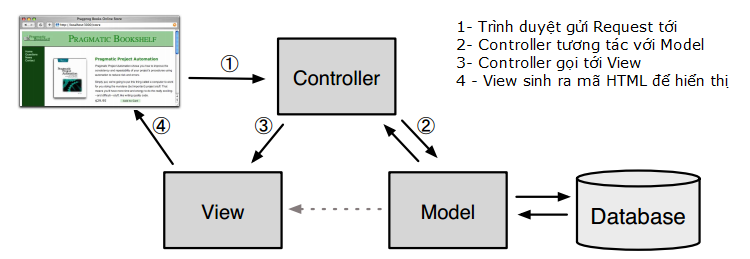
\includegraphics[width=15cm, height=7cm]{image/rails.png}
	\caption{Kiến trúc M-V-C trong  Rails}
	\label{fig:rails}
\end{figure}


\section{Model trong Rails}
Trên thực tế Rails là web framework hướng cơ sở dữ liệu, có nghĩa là database sẽ là phần quan trọng nhất của ứng dựng, chính vì thế Rails có một số thành phần hỗ trợ cho việc xử lý cơ sở dữ liệu và model trở lên dễ dàng hơn.

\subsection{Object-Relational Mapping}
{\bf Object-Relational Mapping} (ORM) là một cơ chế giúp ánh xạ một bảng dữ liệu trong cơ sở dữ liệu quan hệ với một class trong một ngôn ngữ lập trình hướng đối tượng, các dòng trong bảng thành các đối tượng, các cột thành các thuộc tính của đối tượng, và ngược lại.
\newline
Để tránh phải viết nhiều các câu lênh SQL khiến ứng dụng khó bảo trì cơ chế ORM hỗ trợ các phương thức để giao tiếp với cơ sở dữ liệu.
Đối với một số framework khác việc cấu hình giữa cơ sở dữ liệu và model sẽ yêu cầu lập trình viên phải thực hiện, thông thường phải viết và duy trì khá nhiều file cấu hình dạng XML. Trong Rails việc cấu hình 
sẽ không cần phải thực hiện nhờ sự hỗ trợ của thành phần gọi là Active Record.

\subsection{Active Record}
Active Record là một mẫu thiết kế sử dụng trong Object-Relational Mapping, mẫu thiết kế Active Record đưa ra các phương thức cơ bản giúp việc giao tiếp với cơ sở dữ liệu như create, read, update, delete - CRUD. \newline
Trong Rails có một thành phần là Active Record hỗ trợ cơ chế ORM. Về cơ bản thành phần này tuần theo mô hình ORM chuẩn : bảng ánh xạ với class, dòng ánh xạ với đối tượng, cột ánh xạ với thuộc tính. Nhưng cách cấu hình để liên kết giữa cơ sở dữ liệu và model khác biệt. Bằng cách dựa trên các cấu hình quy ước mặc định, Active Record giảm thiểu việc phải viết các file cấu hình.
Chỉ cần một khai báo một class model theo chuẩn của Rails thì model đó sẽ được tự động ánh xạ với một bảng dữ liệu trong cơ sở dữ liệu, cũng như cung cấp ngay các phương thức để giao tiếp với cơ sở dữ liệu. 
Đoạn code ở Listing ~\ref{active-record} sẽ mô tả việc tạo môt model trong Rails cũng như sử dụng các phương thức để thực hiện các thao tác như lưu một bản ghi hay tìm một bản ghi.
\begin{lstlisting}[
language=Ruby,
label=active-record,
inputencoding=utf8,
caption=Active Record trong Rails
]

# Declares a model
class User < ActiveRecord::Base
end
# Initiates an user and stores into database  
user = User.new
user.save
# Finds a user whose id is 1
user = User.find(1)
\end{lstlisting}

Active Record là một thành phần (một module) nền tảng trong kiến trúc M-V-C của Rails.

\section{View và Controller}
View và Controller là 2 thành phần có quan hệ khá chặt chẽ với nhau, controller chuyển dữ liệu từ model để hiển thị trong View, View gửi các sự kiện tới Controller để được xử lý, bởi các sự tương tác này View và Controller được đặt vào trong một thành phần gọi là Action Pack.

\subsection{View}
View trong Rails đơn giản chứa các đoạn mã HTML cho các nội dung cố định, để hiển thị các thông tin động được lấy từ cơ sở dữ liệu, View có thể nhúng các đoạn mã Ruby vào bên trong, được gọi là Embedded Ruby với phần mở rộng là .html.erb. Việc nhúng mã Ruby vào trong View có thể phá vỡ cấu trúc của mô hình MVC nếu các đoạn mã đó chứa các xử lý logic của ứng dụng, vì vậy các đoạn code Ruby nhúng vào chỉ nên dùng để hiển thị thông tin trong Model được cung cấp bởi Controller, các xử lý logic nên được đưa hết vào bên trong Controller và Model. 
 
\subsection{Controller}
Controller là phần trung tâm xử lý các logic của ứng dụng, cộng tác các tương tác giữa người dùng, View, Model với nhau. Việc xây dựng ứng dụng Rails tập trung vào mức xây dựng từng chức năng hoàn chỉnh, việc này giúp việc phát triển và bảo trì rất dễ dàng, mỗi chức năng sẽ được định nghĩa trong Controller.

